\documentclass{beamer}

\usetheme{Antibes}

\title{The Bitcoin Mining Protocol}

\author[Lamur, Duran]{Jules Lamur\inst{1} \and Jeremy Duran\inst{1}}
\institute
{
    \inst{1}
    Université de Toulouse 3 --- Paul Sabatier
}
\date[2019]{English Course Oral Presentation 2019}

\subject{Computer Science}

\AtBeginSection[]
{
    \begin{frame}
        \frametitle{Table of Contents}
        \tableofcontents[
            currentsection,
            hideothersubsections]
    \end{frame}
}

\begin{document}

\frame{\titlepage}

\begin{frame}
    \frametitle{Table of Contents}
    \tableofcontents[hidesubsections]
\end{frame}

\section{Introduction}

\begin{frame}
    \begin{center}
        
\includegraphics[height=3cm]{bitcoin_logo.png}
    \end{center}

    \textbf{Bitcoin} is a crypto-currency based on decentralized consensus rules.
    \pause

    The \textbf{Bitcoin Protocol} is the specification of said rules.
\end{frame}

\subsection{History}

\begin{frame}
    \begin{itemize}
        \item Created in 2008 by \textbf{Satoshi Nakamoto} (anonymous
            individual or group).

        \item Satoshi released, along with the very first Bitcoin
            implementation, a white paper named \textit{Bitcoin: A Peer-to-Peer
            Electronic Cash System}\footnote{https://bitcoin.org/bitcoin.pdf}
            where he describes the purpose and motivations of the Bitcoin
            creation.

        \item A lot of forks exist, \textit{e.g.} Litecoin, Bitcoin Cash,
            Dogecoin. The ``orignal'' Bitcoin implementation is known as
            \textbf{Bitcoin Core}.

        \item Nowadays, the Bitcoin Core source-code is maintained by a lot of
            different people around the world, and all forks follows more or
            less precisely the rules implemented by the Core.
    \end{itemize}
\end{frame}

\section{The Life of a Transaction}

\begin{frame}
    \begin{center}
        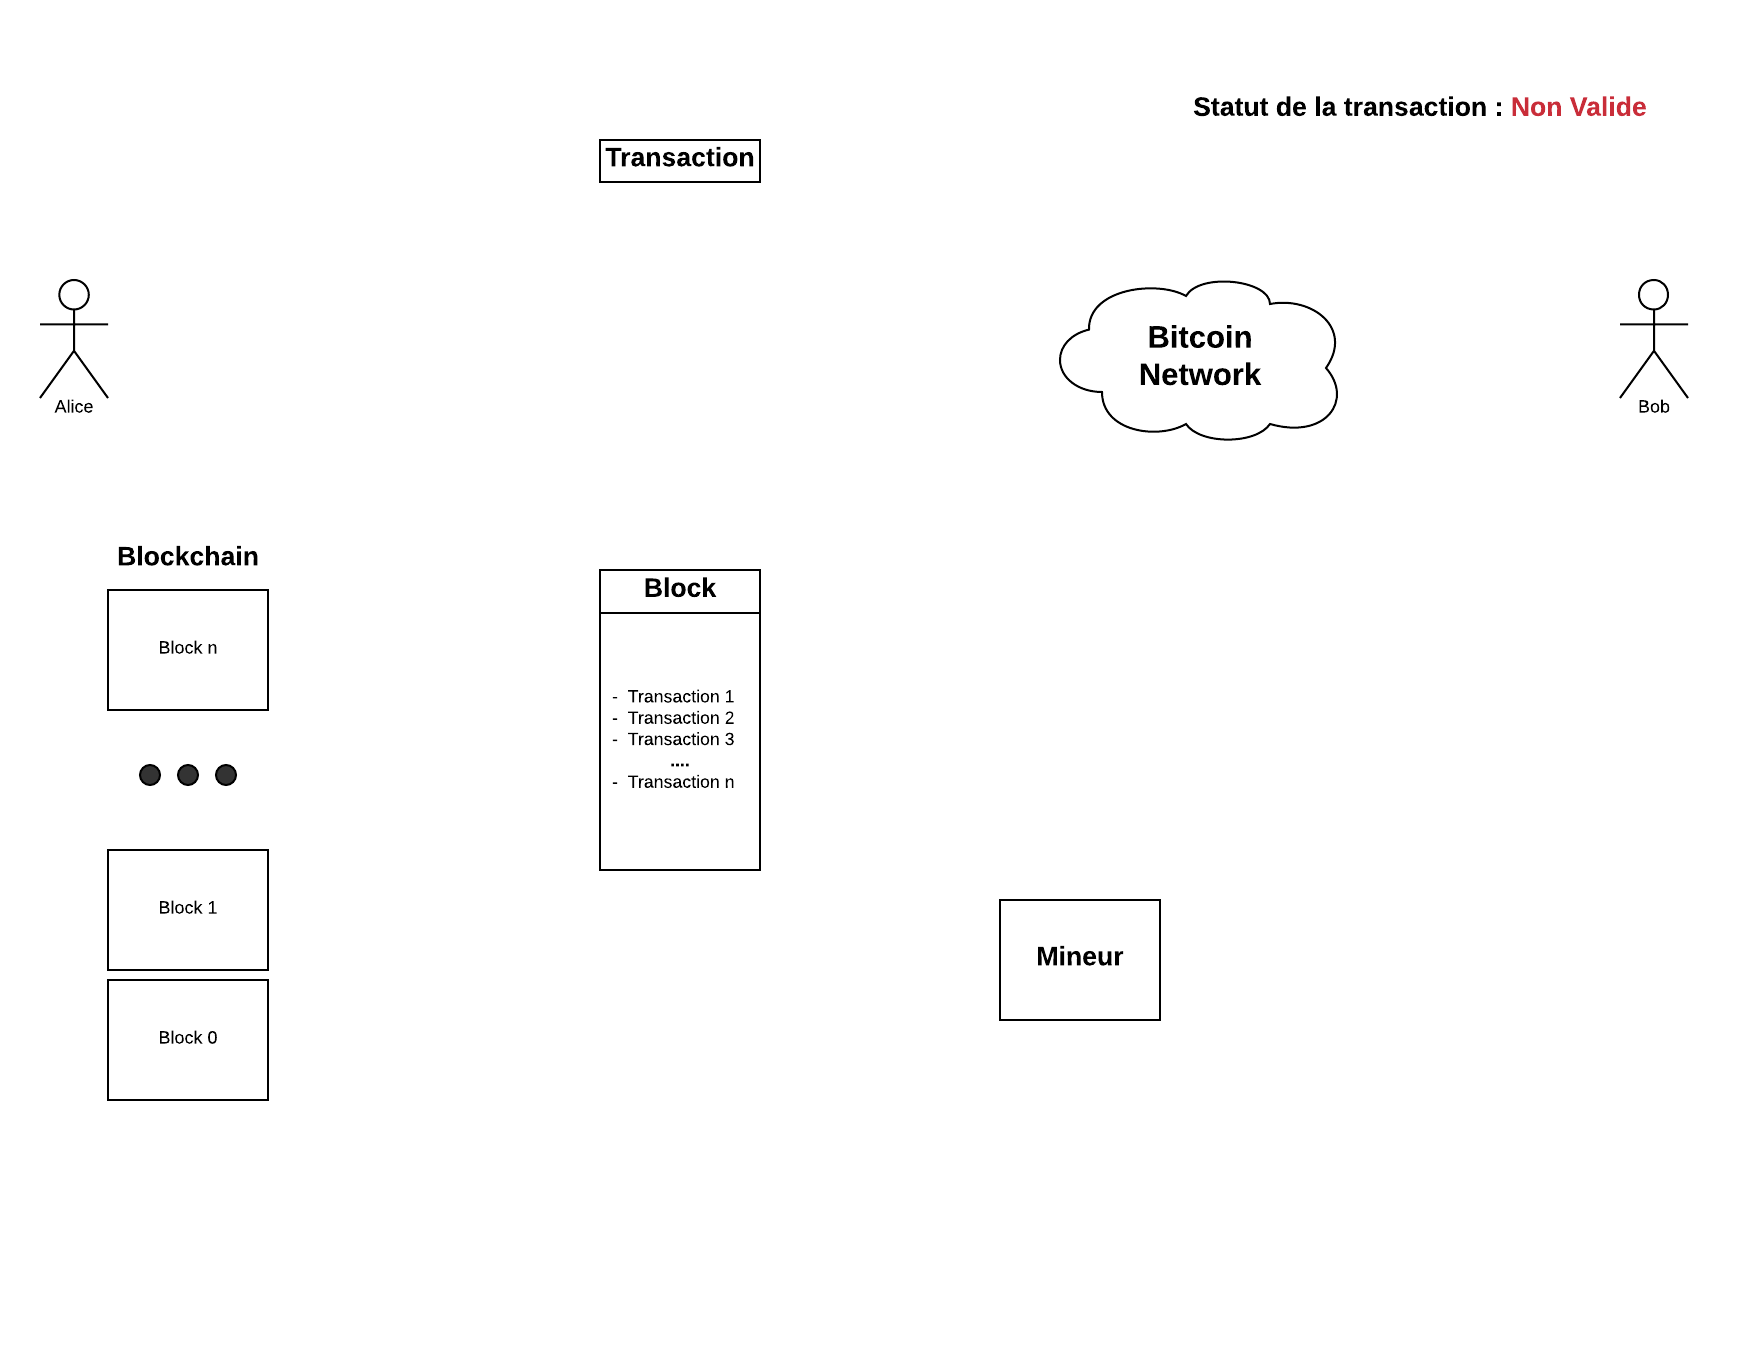
\includegraphics[height=7cm]{images/explanation-0.png}
    \end{center}
\end{frame}

\begin{frame}
    \begin{center}
        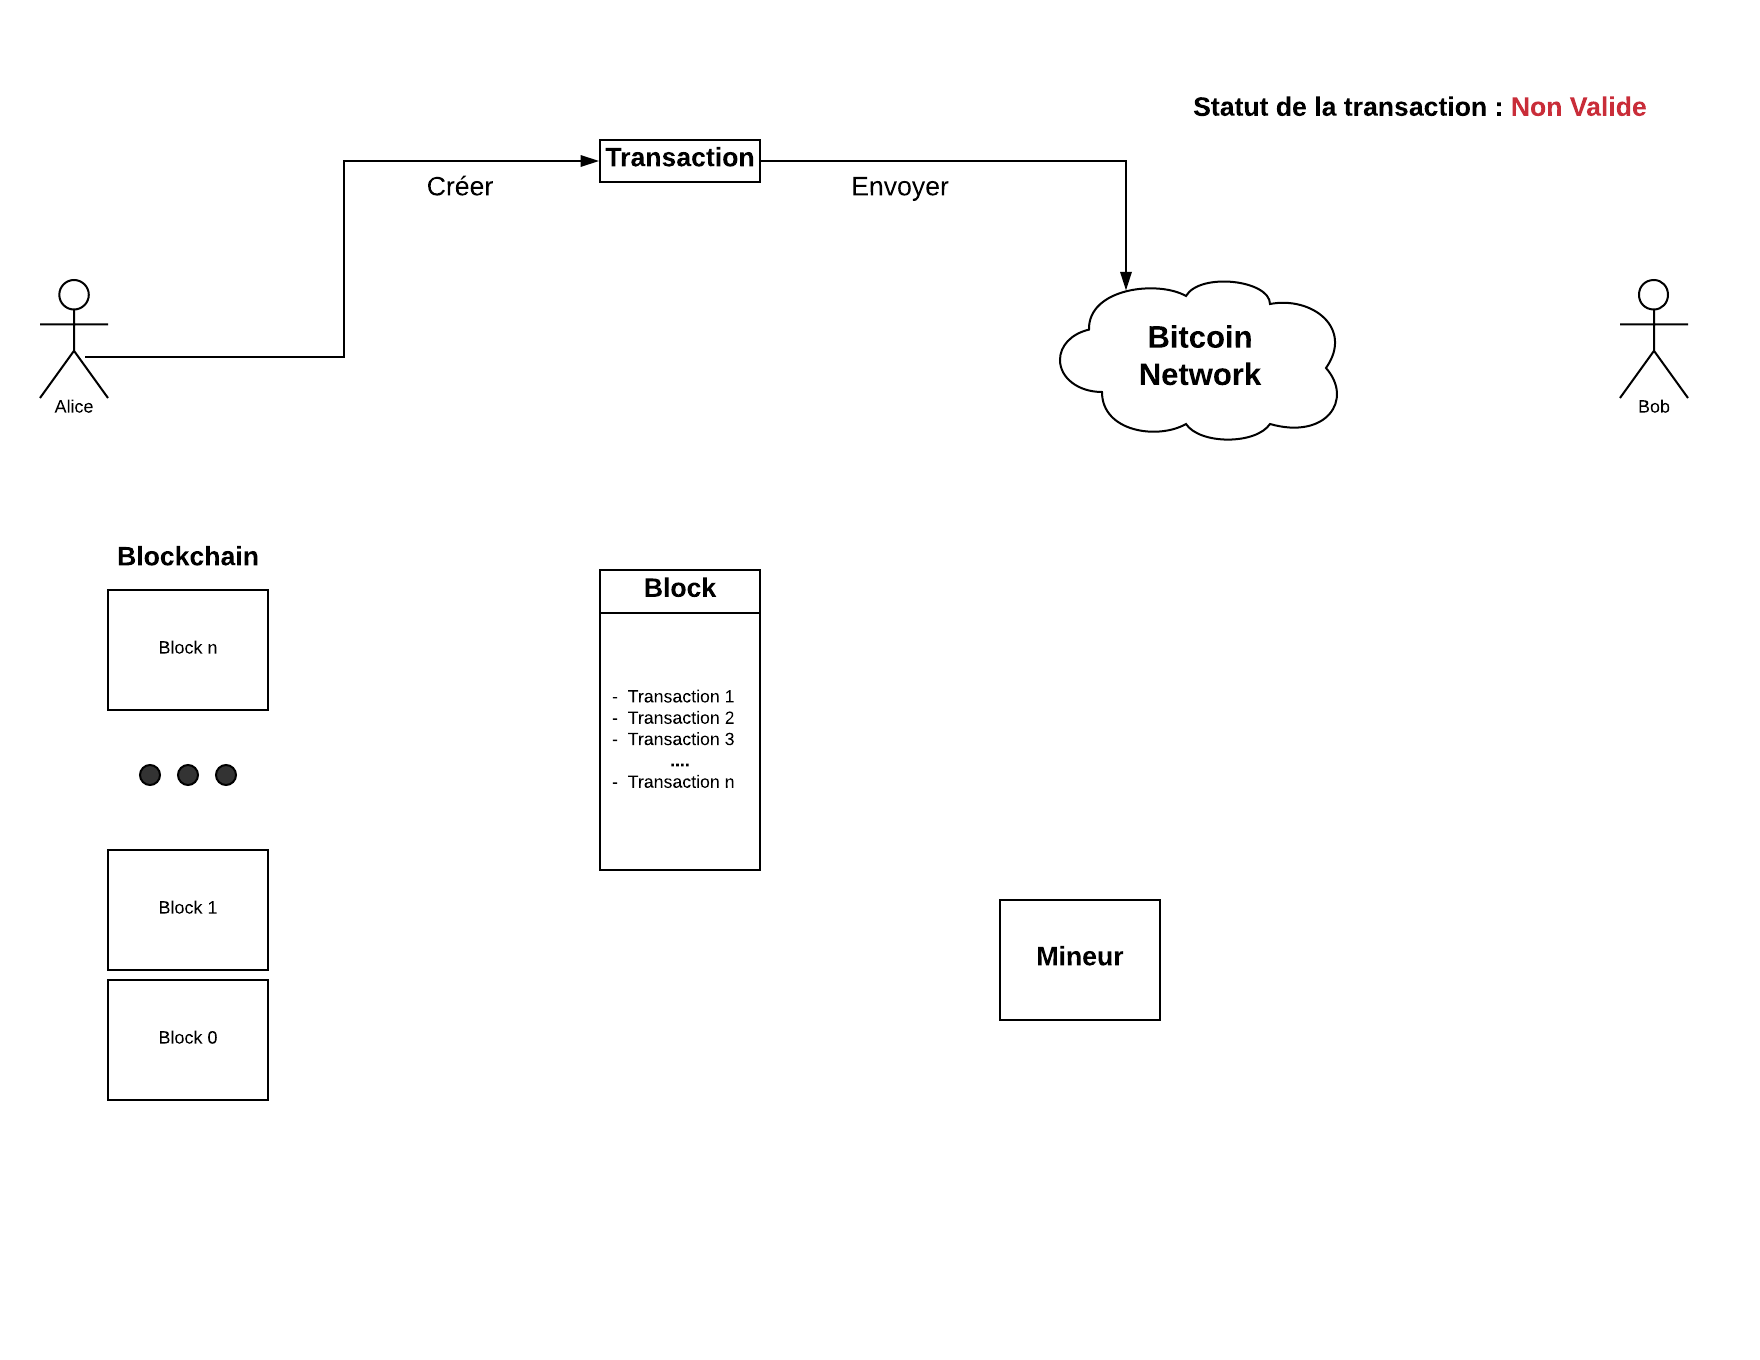
\includegraphics[height=7cm]{images/explanation-2.png}
    \end{center}
\end{frame}

\begin{frame}
    \begin{block}{Asymetric cryptography}
        Works with public keys ($p_k$) and private keys ($s_k$)
        \pause
        \begin{itemize}
            \item public keys are know to the general public
            \item private keys are only know to the user
                \pause
        \end{itemize}
        Sign(message,$p_k$) = Signature

        \pause
        Verify(message,Signature,$p_k$) = True/False
    \end{block}
\end{frame}


\begin{frame}
    \begin{center}
        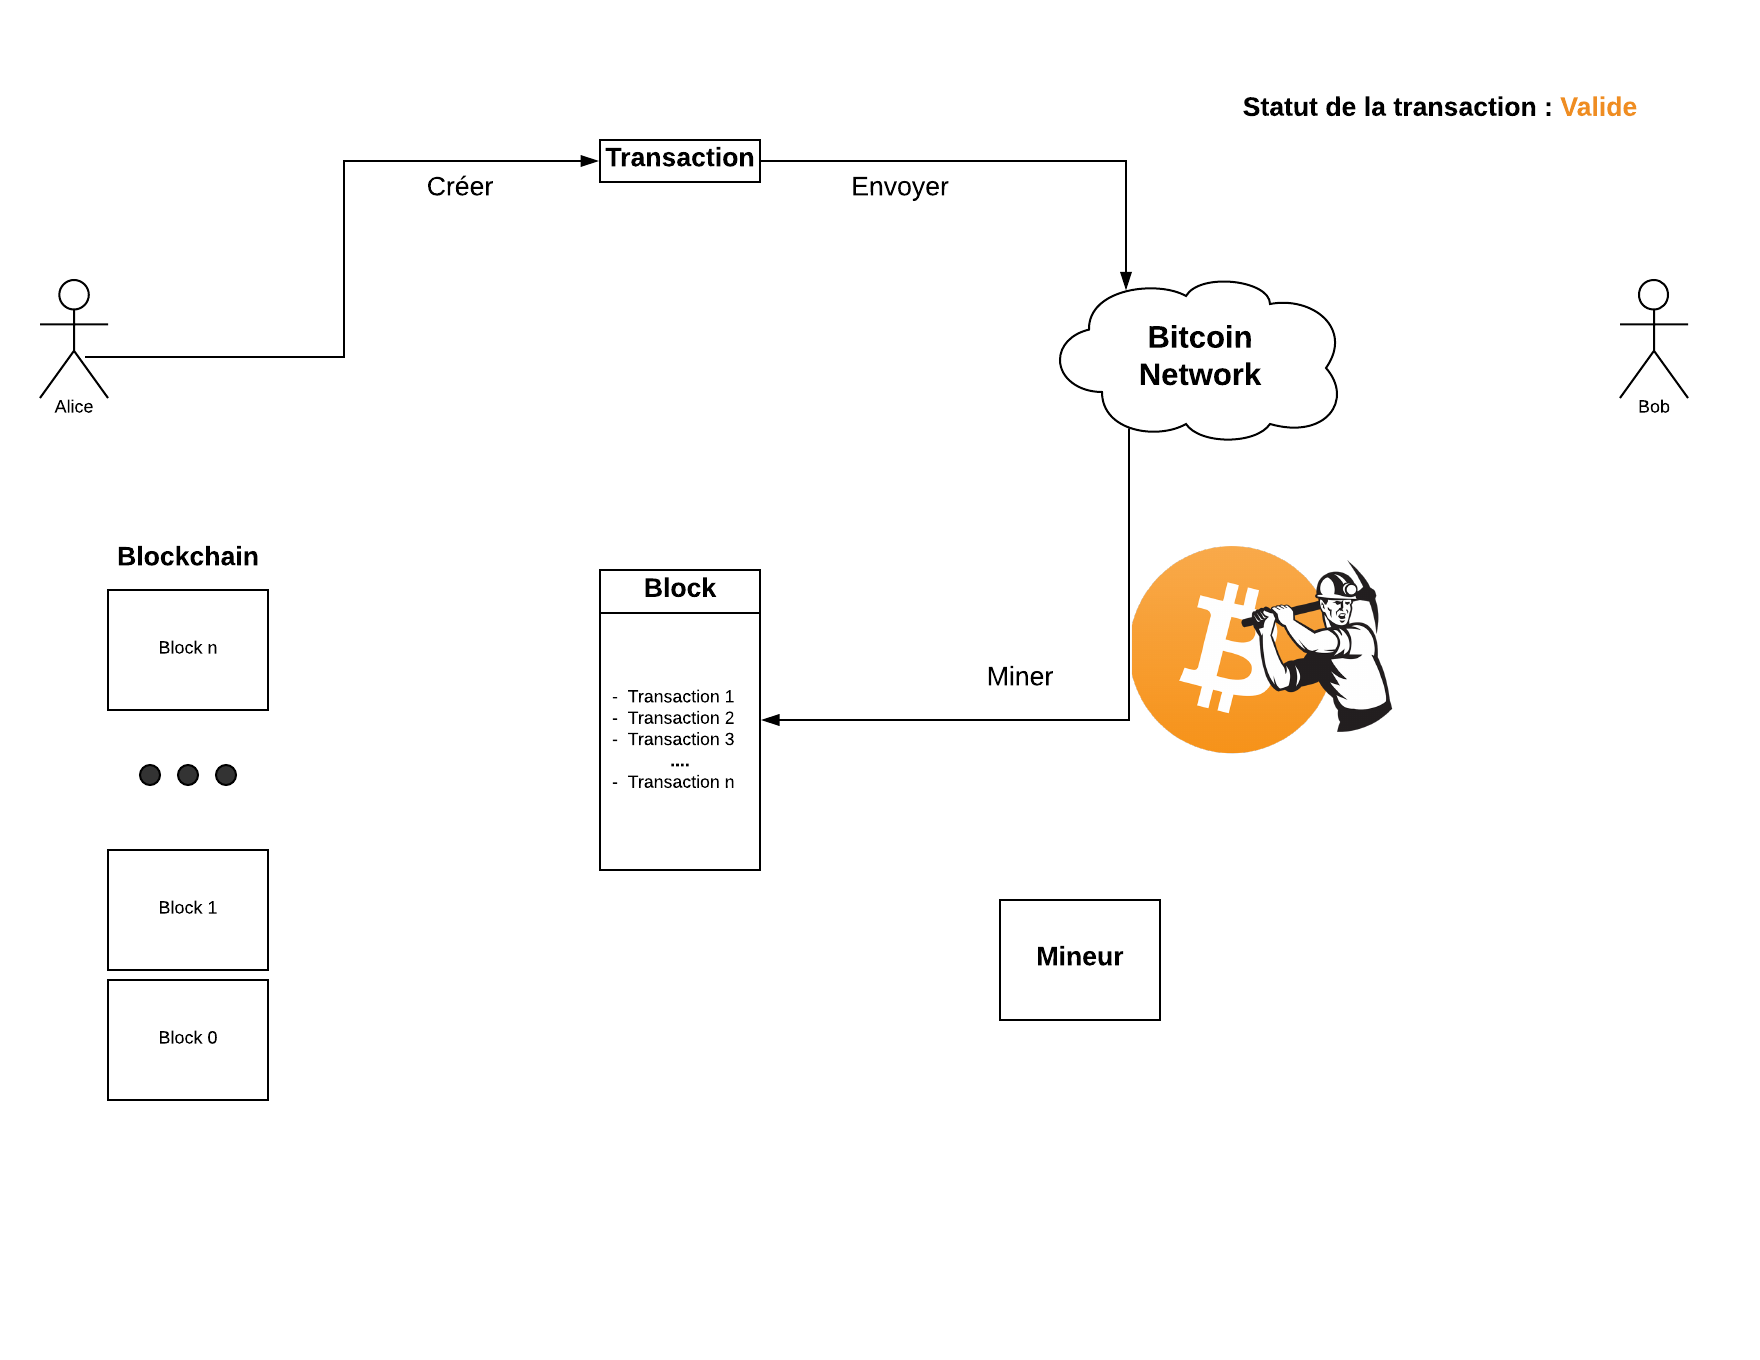
\includegraphics[height=7cm]{images/explanation-3.png}
    \end{center}
\end{frame}

\begin{frame}
    \begin{center}
        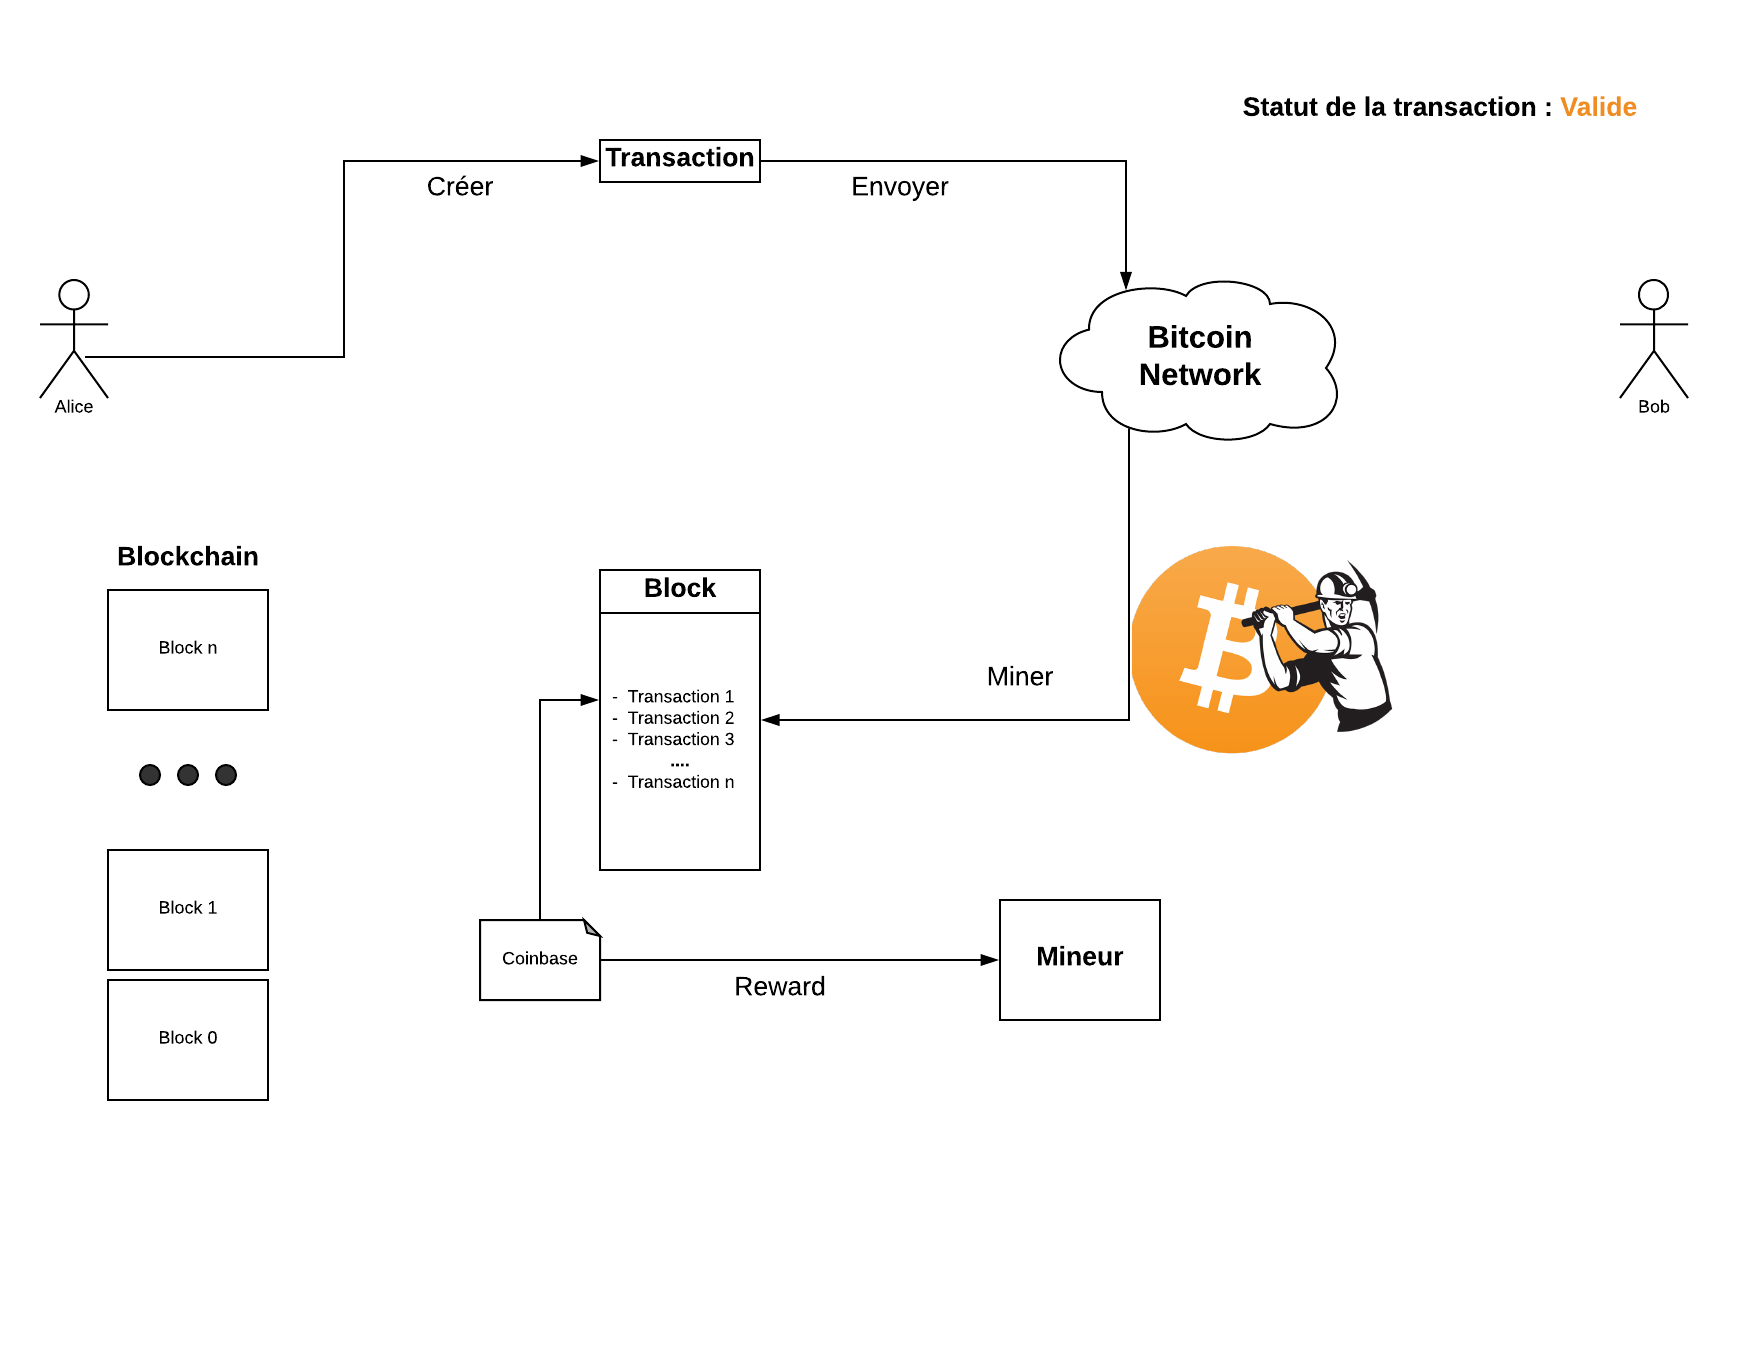
\includegraphics[height=7cm]{images/explanation-4.png}
    \end{center}
\end{frame}

\begin{frame}
    \begin{center}
        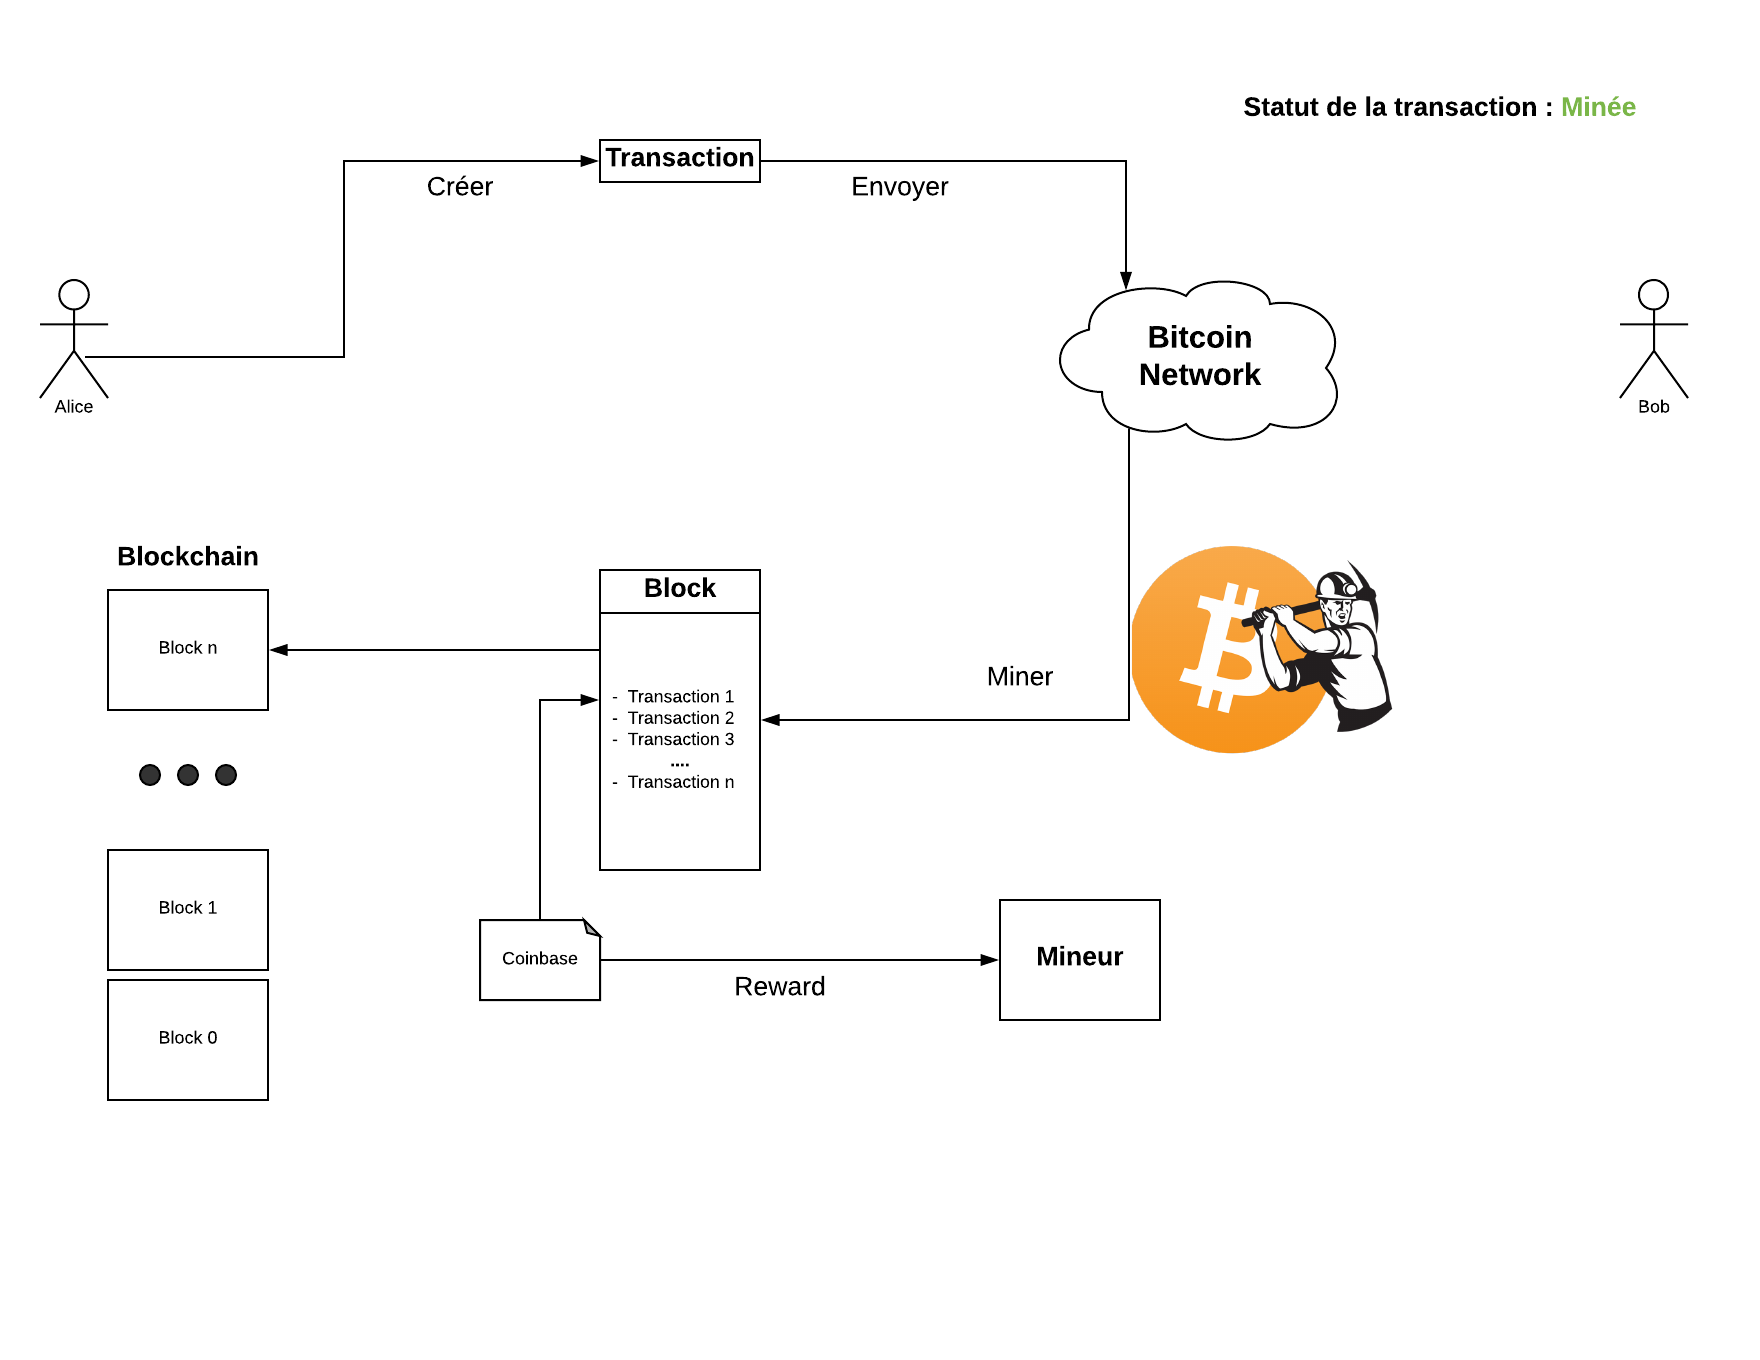
\includegraphics[height=7cm]{images/explanation-5.png}
    \end{center}
\end{frame}

\begin{frame}
    \begin{center}
        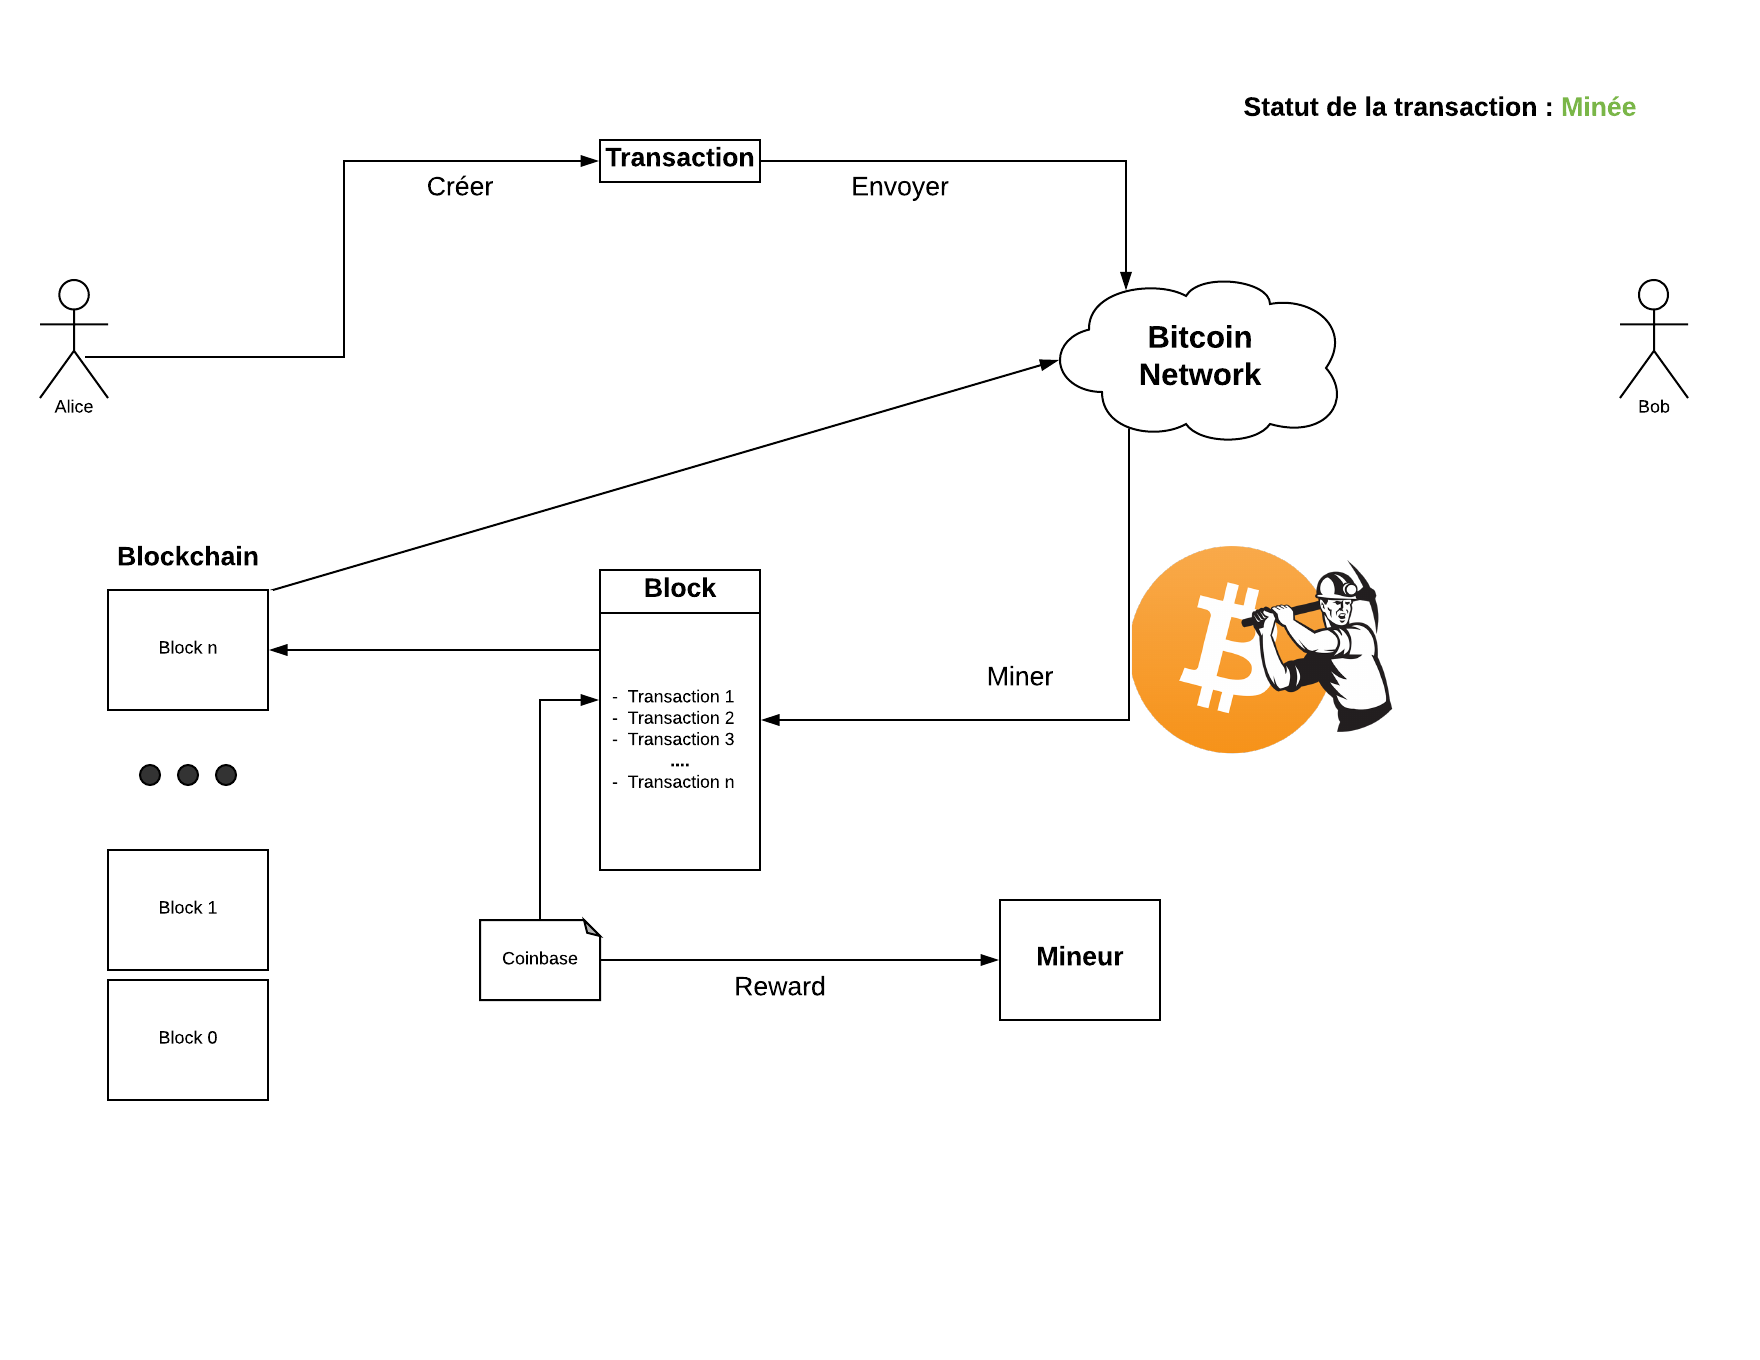
\includegraphics[height=7cm]{images/explanation-6.png}
    \end{center}
\end{frame}

\begin{frame}
    \begin{center}
        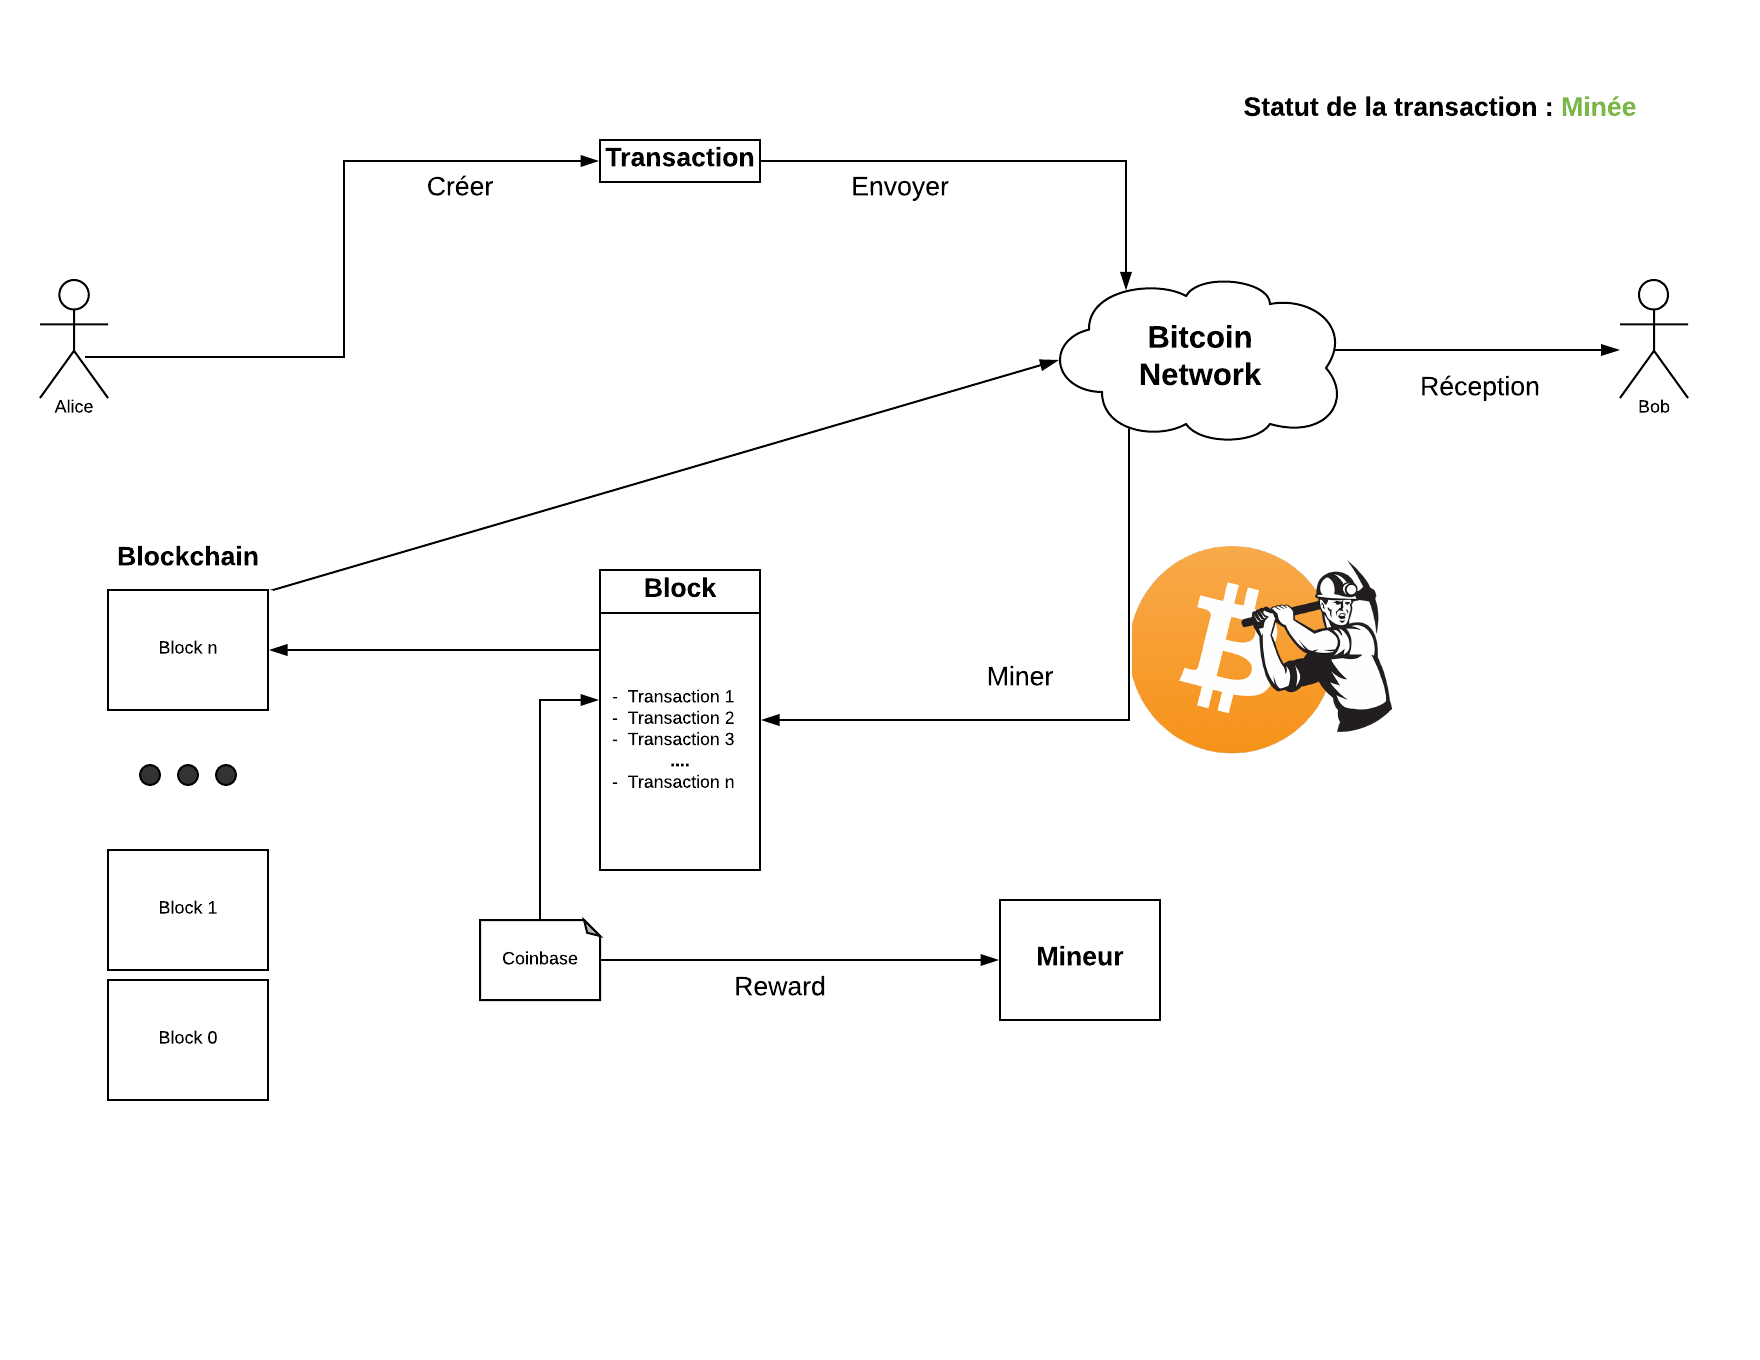
\includegraphics[height=7cm]{images/explanation-7.png}
    \end{center}
\end{frame}

\begin{frame}
    \begin{center}
        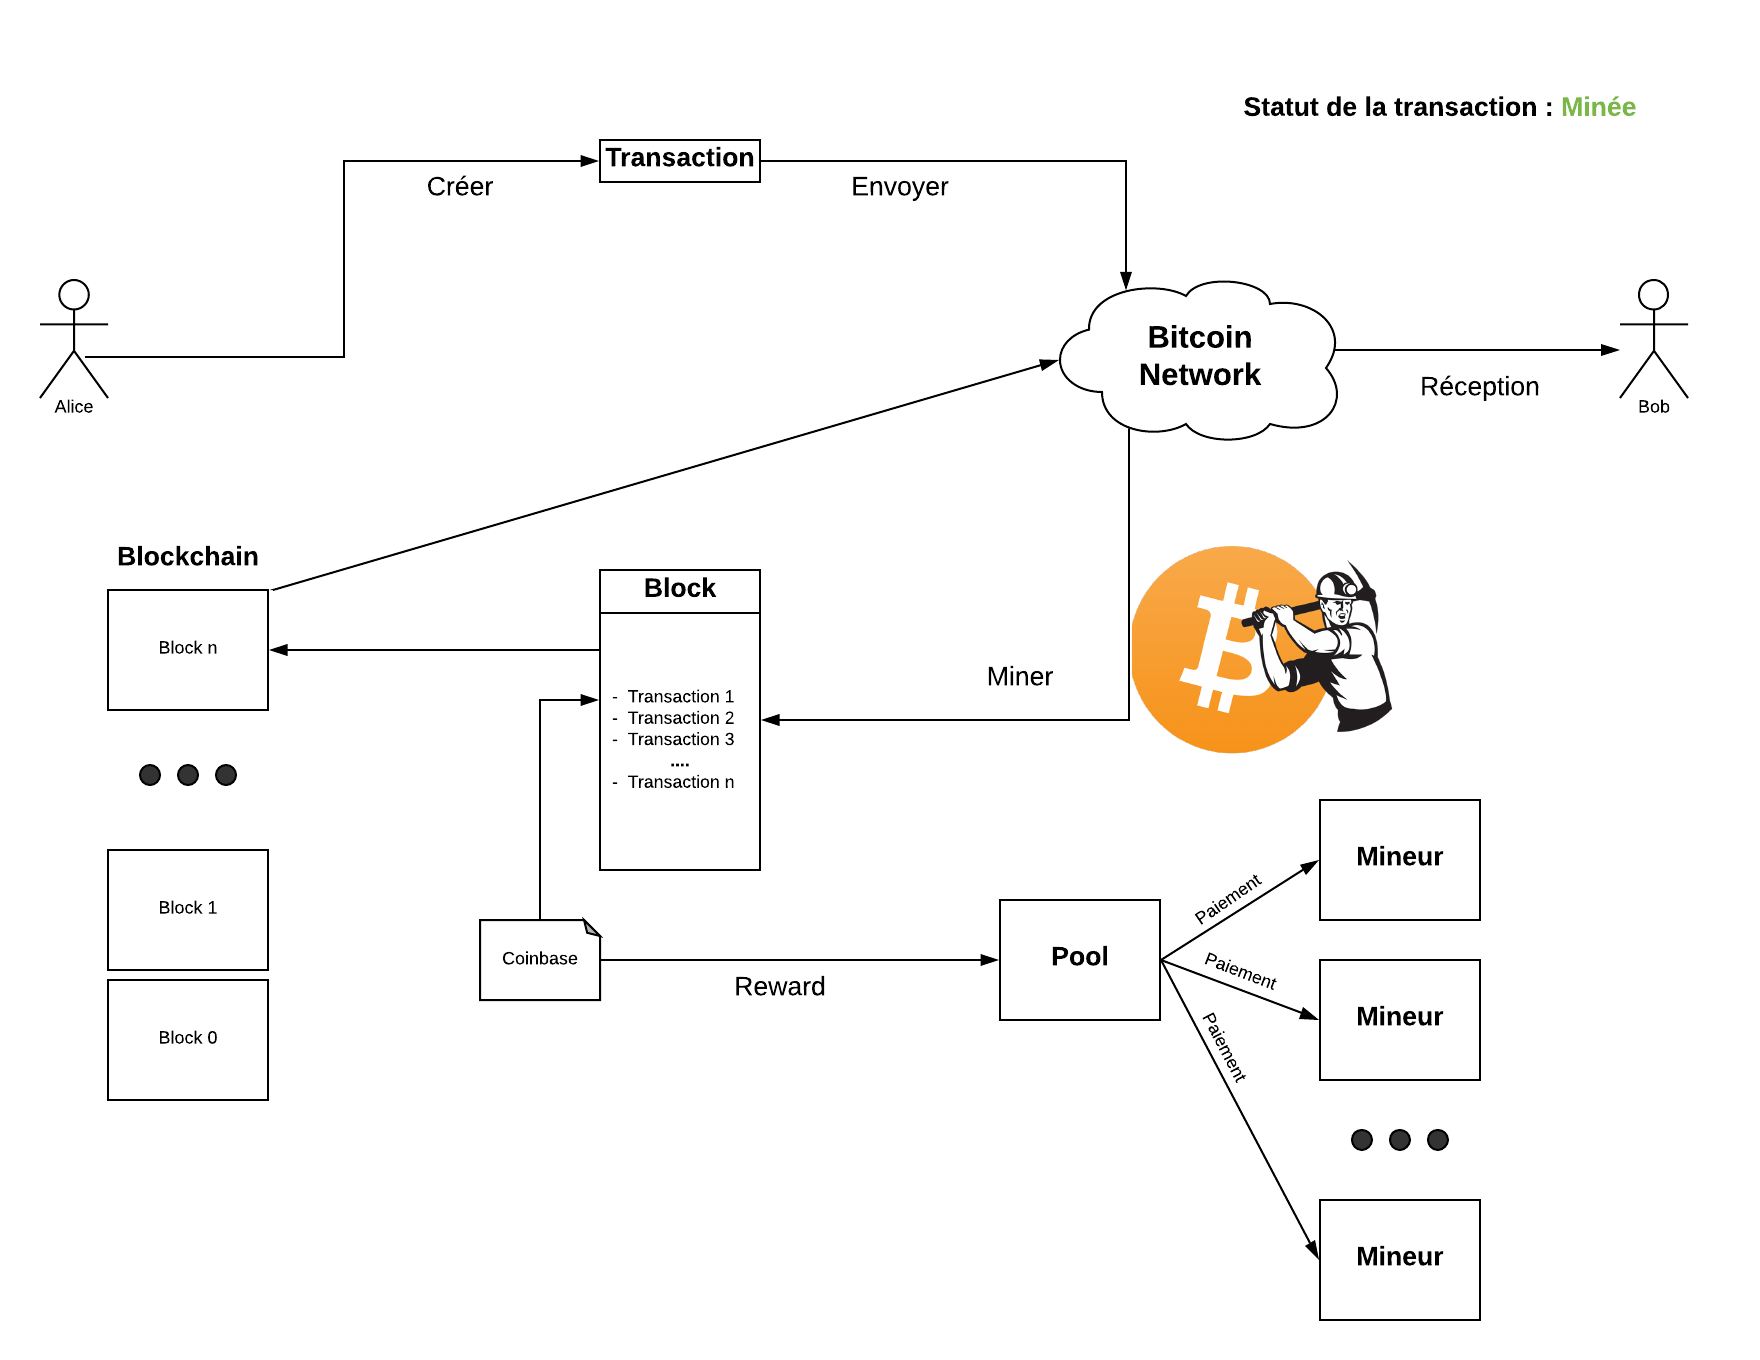
\includegraphics[height=7cm]{images/explanation-8.png}
    \end{center}
\end{frame}

\section{Mining}
\subsection{Prerequisites}

\begin{frame}
    \begin{block}{Hash function}
        The ideal cryptographic hash function has five main properties:
        \begin{itemize}
            \item Deterministic the same message always results in the same hash
            \item Quick to compute
            \item Infeasible to generate a message from its hash value except by trying all possible messages
            \item A small change changes the entire hash value
            \item Infeasible to find two different messages with the same hash values
        \end{itemize}
    \end{block}
\end{frame}
\begin{frame}
    A couple hash functions:
    \begin{itemize}
        \item MD5 (128 bits) \pause \textbf{broken} \pause
        \item SHA-1 (160 bits) \pause \textbf{broken} \pause
        \item SHA-2 (e.g. SHA-256 and SHA-512) \pause \textbf{not broken} \pause
        \item and many more
    \end{itemize}
    \pause
    The main hash function used by Bitcoin: SHA-256.
\end{frame}

\subsection{Proof of Work}
\begin{frame}
    A block is valid if its hash is less than the target difficulty.

    \pause
    Example:
    \begin{block}{Bitcoin Block \#2}
        \begin{tabular}{ r l }
            Hash: &   \texttt{000000006a625f06636b8bb6ac7b960a8d03705}\ldots \\
            Target: & \texttt{00000000ffff000000000000000000000000000}\ldots \\
            Difficulty: & 1 \\
            Nonce: & 1639830024
        \end{tabular}
    \end{block}

    \pause
    \begin{itemize}
        \item Hash $\leq$ Difficulty $\implies$ Block is valid
        \item Target $\iff$ Difficulty
        \item Nonce is a free field: miners iterate throught a lot of them to
            get different hashes.
    \end{itemize}

    \pause
    Difficulty is adjusted every 2 weeks in order to keep a 10 minute average
    between blocks.

    \pause
    Todays difficulty is around 6,393,023,717,201.86.
\end{frame}

\section{Transaction Scripts}
\begin{frame}
    Transactions are not payments \pause but actually scripts.

    \pause
    Some of the scripts are standardized and are actual payments.

    \pause
    The Lightning Network is an application that uses transaction scripts.
\end{frame}

\end{document}
